\documentclass[11pt]{article}

\usepackage[margin=1in]{geometry}
\usepackage{amsfonts, amsmath, amssymb}
\usepackage[none]{hyphenat}
\usepackage{fancyhdr}
\usepackage{graphicx}
\usepackage{float}
\usepackage{mathtools}
\usepackage{enumitem}
\usepackage{comment}
\usepackage[nottoc, notlot, notlof]{tocbibind}

\pagestyle{fancy}
\fancyhead{}
\fancyfoot{}
\fancyhead[L]{\slshape\MakeUppercase{Método de Newton para sistemas no lineales}}
%\fancyhead[R]{\slshape{Student Name}}
\fancyfoot[C]{\thepage}
%\renewcommand{\headrulewidth}{0pt}
\renewcommand{\footrulewidth}{0pt}

\DeclarePairedDelimiter\abs{\lvert}{\rvert}%
\DeclarePairedDelimiter\norm{\lVert}{\rVert}%

% Swap the definition of \abs* and \norm*, so that \abs
% and \norm resizes the size of the brackets, and the 
% starred version does not.
\makeatletter
\let\oldabs\abs
\def\abs{\@ifstar{\oldabs}{\oldabs*}}
%
\let\oldnorm\norm
\def\norm{\@ifstar{\oldnorm}{\oldnorm*}}
\makeatother

\parindent 0ex
%\setlength{\parindent}{4em}
%\setlength{\parskip}{1em}
\renewcommand{\baselinestretch}{1.5}

\begin{document}
\begin{titlepage}

\begin{center}
%\vspace*{1cm}
\Large{\textbf{Análisis Numérico}}\\
\Large{\textbf{Proyecto Final}}\\
\vfill
\line(1,0){500}\\[1mm]

\huge{\textbf{Método de Newton para sistemas no lineales}}\\[3mm]
\Large{\textbf{- Implementación y teoría del método -}}\\[1mm]

\line(1,0){500}\\
\vfill
00076015 Carlos Javier Burgos Martinez\\
00006715 David Bejamín Ayala Giralt\\
00388913 Diego José Eguizabal Liu\\
00058615 Karla Esperanza López Méndez\\
00353715 Mario Cecilio De Leon Recinos\\
00004315 Rafael Enrique Cruz Aparicio \\
00088116 Yury Alejandro Rivera Quintanilla\\
\vfill
\today\\

\end{center}

\end{titlepage}

\tableofcontents
\thispagestyle{empty}
\clearpage

\setcounter{page}{1}

\section{Definiciones}

El problema computacional que se intenta resolver es encontrar soluciones para ecuaciones de sistemas no lineales. Las cuales seran resueltas con el metodo de newton adaptado para sistemas no lineales. Este metodo ha sido modificado de tal forma que el algoritmico
pueda efectuar la transformacion a un sitema de $\mathbb{R}^{n}$ .\\

Para construir dicho algoritmo que lleve a una solución del método de punto-fijo en un caso unidimensional, obtuvimos una función $\phi$ con las propiedades $$g(x)=x-\phi(x)f(x)$$ que da una convergencia cuadrática en el punto fijo $p$ de la función $g$.De esta condición el método de Newton evolucionó al escoger $\phi(x)=1/f'(x)$ asumiendo que $f'(x)\neq0$.\\

Un enfoque similar en el caso $n$-dimensional implica una matriz:

\begin{equation}
A=
\begin{bmatrix}
    a_{11}       & a_{12} & \dots & a_{1n} \\
    a_{21}       & a_{22} & \dots & a_{2n} \\
    \vdots & \vdots & \ddots  & \vdots\\
    a_{n1}       & a_{n2} & \dots & a_{nn}
    \label{matrix:A}    
\end{bmatrix}
\end{equation}


Donde cada una de las entradas $a_{ij}(x)$ es una función de $\mathbb{R}^n$ a $\mathbb{R}$ . Esto requiere que $A(x)$ sea encontrado para que $$\mathbf{G(x)=x-A(x)^{-1}F(x)}$$ genere una convergencia cuadrática para la solución $\mathbf{F(x)=0}$, asumiendo que $A(x)$ es no singular en el punto fijo $\mathbf{p}$ de $\mathbf{G}$.\\

Suponemos que $p$ es una solución de $G(x)=x$. Si existe un número $\delta>0$ con la propiedad que:

\begin{enumerate}[label=(\roman*)]

	\item $\partial g_i / \partial x_j$ sea continua en $N_\delta=x|\quad \norm{x-p}$ para toda $i=1,2,...,n$ y toda $j=1,2,///,n;$
	\item $\partial^2 g_i(x) / \partial x_j\partial x_k$ sea continua y $\abs{ \partial^2 g_i(x)/(\partial x_j\partial x_k)}\leq M$ para alguna constante M siempre que $x\in N_\delta$ para toda $i=1,2,...,n, j=1,2,...,n$ y toda $k=1,2,...,n;$ 
	\item $\partial g_i(p) /\partial x_k =0$ para toda $i=1,2,...,n$ y toda $k=1,2,...,n.$

\end{enumerate}

Entonces existe un número $\hat{\delta}\leq \delta$ tal que la sucesión generada por $x^k=G(x^{k-1})$
converge cuadráticamente a $p$ para cualquier elección de $x^0$ a condición de que $\quad \norm{x^0-p}<\hat{\delta}$
\begin{center}
$\quad \norm{x^k-p}_\infty \leq \frac{n^2M}{2}\quad \norm{x^{k-1}-p}_\infty^2$ para toda k$\geq 1$
\end{center}
Para utilizar el teorema supongamos que $A(x)$ es una matriz de $n X n$ de funciones de $\mathbb{R}^n$ a $\mathbb{R}$ en la forma de la ecuación \ref{matrix:A}, cuyos elementos específicos se escogerán más adelante. Supongamos además que $A(x)$ es no singular cerca de una solución $p$ de $F(x)=O$ , y denotemos con $b_{ij}(x)$ el elemento de $A(x)^{-1}$ en el i-ésimo renglón y en la j-ésima columna.

Dado que $G(x)=x-A(x)^{-1}F(x)$, tenemos $g_i(x)=x_i-\sum_{j=1}^{n}b_{ij}(x)f_{j}(x)$
\begin{equation}
\centering
\label{tab:data1}
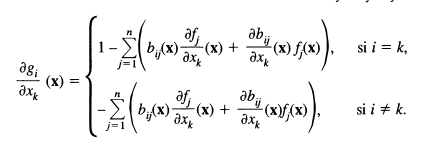
\includegraphics[scale=1.0]{jacobianos}
\end{equation}

El teorema que se menciono anteriormente implica que necesitamos $\partial g_i(p)/\partial x_k$ para toda $i=1,2,...,n$ y toda $k=1,2,...,n$. Esto significa que, para toda $i=k$,

$$0=1-\sum_{j=1}^{n}b_{ij}(p){\frac{\partial f_{j}}{\partial x_{i}}(p)},$$
por lo que
\begin{equation}
\sum_{j=1}^{n}b_{ij}(p){\frac{\partial f_{j}}{\partial x_{i}}(p)}=1
\label{eq:sindespejar}
\end{equation}

\qquad Cuando $k\neq1$


$$0=-\sum_{j=1}^{n}b_{ij}(p){\frac{\partial f_{j}}{\partial x_{i}}(p)}$$

por lo que 
\begin{equation}
\sum_{j=1}^{n}b_{ij}(p){\frac{\partial f_{j}}{\partial x_{i}}(p)}=0
\label{eq:despejada}
\end{equation}
Al definir la matriz $J(x)$ por medio de
\begin{equation}
J=
\begin{bmatrix}
    \frac{\partial f_1}{\partial x_1}(x)       & \frac{\partial f_1}{\partial x_2}(x)       & \dots & \frac{\partial f_1}{\partial x_n}(x)       \\
    \frac{\partial f_2}{\partial x_1}(x)             & \frac{\partial f_2}{\partial x_2}(x)       & \dots & \frac{\partial f_2}{\partial x_n}(x)       \\
    \vdots & \vdots & \ddots  & \vdots\\
    \frac{\partial f_n}{\partial x_1}(x)             & \frac{\partial f_n}{\partial x_2}(x)       & \dots & \frac{\partial f_n}{\partial x_n}(x)      
    \label{matrix:J}    
\end{bmatrix}
\end{equation}
vemos que las condiciones de las ecuacions (\ref{eq:sindespejar}) y (\ref{eq:despejada}) 
requieren $$A(p)^{-1}J(p)=I, \textrm{la matriz identidad},$$por lo que $$A(p)=J(p).$$
En consecuencia, una eleccion apropiada de $A(x)$ es $A(x)=J(x),$ dado que entonces se cumple la condicion$(iii)$ del teorema.\\
La funcion $G$ esta definida por $$G(x)=x-{J(x)}^{-1}F(x)$$
y el procedimiento de la iteracion funcional pasa de seleccionar $x^0$ a generar, para $k\geq 1,$ $$x^k=G(x^{k-1})=x^{k-1}-{J(x^{k-1})}^{-1}F(x^{k-1})$$
Con esto se concluye que esto es metodo de Newton para sistemas no lineales, y generalmente se espera que de una convergencia cuadratica, siempre y cuando se conozca un valor inicial suficientemente preciso y exista ${J(p)}^{-1}$.\\
La debilidad de este metodo es que se tiene la necesidad de calcular e invertir la matriz $J(x)$ en cada paso.\\
Matriz Jacobiana: Es una matriz que está conformada por las derivadas parciales, de primer orden de una función.
$$
J=
\begin{bmatrix}
    \frac{\partial f_1}{\partial x_1}(x)       & \frac{\partial f_1}{\partial x_2}(x)       & \dots & \frac{\partial f_1}{\partial x_n}(x)       \\
    \frac{\partial f_2}{\partial x_1}(x)             & \frac{\partial f_2}{\partial x_2}(x)       & \dots & \frac{\partial f_2}{\partial x_n}(x)       \\
    \vdots & \vdots & \ddots  & \vdots\\
    \frac{\partial f_n}{\partial x_1}(x)             & \frac{\partial f_n}{\partial x_2}(x)       & \dots & \frac{\partial f_n}{\partial x_n}(x)         
\end{bmatrix}
$$
Campo vectorial es una función vectorial de varias variables en la que a cada punto de su dominio se le asigna el vector correspondiente a una determinada magnitud vectorial que actúa sobre dicho punto.$$F:A\subset\mathbb{R}^n \longrightarrow \mathbb{R}$$ 
Espacio vectorial es la estructura matemática que se crea a partir de un conjunto no vacío y que cumple con diversos requisitos y propiedades iniciales. Esta estructura surge mediante una operación de suma (interna al conjunto) y una operación de producto entre dicho conjunto y un cuerpo.
$$\mathbb{R}_n={x_1,x_1,...,x_n},\textrm{ con } x_i\in \mathbb{R}$$
En $\mathbb{R}_n$, la suma de vectores y el producto por un escalar se definen asi:
$$\textrm{Sean } u=u_1,u_2,...,u_n \textrm{ y }  v_1,v_2,...,v_n \in \mathbb{R}_n$$
$$u+v=(u_1+v_1,u_2+v_2,...,u_n+v_n)\in \mathbb{R}_n$$
$$\alpha v=\alpha v_1,\alpha v_2,...,\alpha v_3 \in \mathbb{R}_n$$
Vector nulo:Es el vector de coordenadas (0,0). O bien, se define como el vector de longitud o módulo cero. La definición de vector nulo es una convención matemática útil para resolver ecuaciones vectoriales. Juega el papel de elemento neutro para la suma de vectores.\\

Matriz inversa: En matemáticas, en particular en álgebra lineal, una matriz cuadrada A de orden n se dice que es invertible, no singular, no degenerada o regular si existe otra matriz cuadrada de orden n, llamada matriz inversa de $A$ y representada como $A^{-1}$, tal que:
$$\begin{bmatrix} 1 & 1 \\ 0 & 1 \\ \end{bmatrix}^{-1} = \begin{bmatrix} 1 & -1 \\ 0 & 1 \\ \end{bmatrix}.$$
 ,donde In es la matriz identidad de orden n y el producto utilizado es el producto de matrices usual.\\
 \\El conjunto $\mathbb{R}_n$ es el producto cartesiano $\mathbb{R}x...x\mathbb{R}=\mathbb{R}_n$, cuyos elementos son las n-uplas de números reales $(x_1,...,x_n), x_1 \in \mathbb{R},i=1,...,n$, llamados vectores de n componentes.


\section{Desarrollo del programa}
Este programa fue desarrollado con la intención de permitir resolver sistemas de ecuaciones no lineales, de manera numérica, usando el método de Newton adaptado para estos tipos de sistemas. Estos sistemas son un conjunto de ecuaciones no lineales que tienen múltiples variables y describen fenómenos bastante complejos como los simulados por computadora.

\subsection{Algoritmo}
El algoritmo que utilizamos en este caso fue el  método de Newton adaptado para trabajar con sistemas no lineales de $n$ funciones y $n$ variables que mapean $\mathbb{R}^3$ a $\mathbb{R}^3$ de forma iterativa. Como ya se mencionó en esta forma, el método de Newton debe trabajar para resolver varias ecuaciones con varias incógnitas es decir, un sistema de ecuaciones. La característica principal de este sistema es ser no lineal, por lo que los métodos convencionales para resolver el SEL resultan ser no útiles. A consecuencia de esto se necesita otro tipo de método. Uno de los candidatos es el método de Newton, sin embargo este método esta definido para una variable y se deduce de un polinomio de series de potencias, un polinomio de taylor de segundo grado para ser precisos. Por lo que, este método no puede aplicarse directamente al sistema y necesita ser adaptado. Describimos los cambios de forma general a continuación.\\

Si recordamos la forma unidimensional del método de Newton:\\
\begin{center}
$x_{k+1} = x_{k} + \frac{f(x_{k})}{f^\prime(x_{k})} \label{eq:1}$\\
\end{center}

Se observa que cada iteración está dada por el valor resultante de la iteración anterior o del valor inicial, más la función evaluada en ese mismo punto, dividido entre la derivada de la función evaluada en ese mismo punto nuevamente. El primer cambio necesario para usar el método de Newton en un sistema no lineal es definirlo de forma matricial, esto se logra desarrollando una aproximación por polinomio de taylor de grado 2 a la función $f(x_{0},x_{1},x_{3},...x_{n})$. De este último polinomio agrupamos todas las derivadas parciales y las convertimos a una forma matricial, generando así la matriz Jacobiana que al invertirla juega el mismo papel que la derivada de la función para el caso unidimensional o el método de Newton sin adaptar. El siguiente cambio importante, es que ya no se itera sobre un punto si no sobre dos vectores columna, el primero que contiene las coordenadas del punto de la iteración anterior o de la inicial y el segundo es un vector con las coordenadas imágenes de $f(x_{n})$.\\
El método adaptado para resolver sistemas de ecuaciones no lineales aún posee una forma y características similares a la de su forma inicial. La diferencia radica en que el método generalizado no trabaja iterando sobre $\mathbb{R}$ para encontrar la raíz de $f$ sino que este itera sobre un campo vectorial de $\mathbb{R}^n$ definido por las $n$ funciones que necesita resolver. En otras palabras el método retorna como respuesta un vector columna con las soluciones o el vector solución.\\

Forma generarizada del método de Newton.
 
\begin{center}
$\bar{X}_{k+1} = \bar{X}_{k} + {J(\bar{X})}^{-1}F(\bar{X})  \label{eq:2}$
\end{center}

Pero para este caso el papel de la derivada lo juega la matriz de derivadas parciales de cada función, es decir, la matriz Jacobiana que nos permite mapear  $\mathbb{R}^3$ a $\mathbb{R}^3$ y en lugar iterar sobre un punto $x$ de $\mathbb{R}$  ahora iteramos en el vector $\bar{X}$. 

Desafortunadamente, el cálculo de una matriz Jacobiana luego debe ser invertido y el cálculo de una matriz inversa resulta demasiado costoso en términos de procesamiento por lo que se optó por usar una forma alternativa al método que genera un SEL al final el cual, es mucho más rápido de resolver\\

\begin{center}
$J(\bar{X}_{k})y = -F(\bar{X}_{k}) $
\end{center}

Siendo $y$ un vector que satisfaga la igualdad, es de la necesidad de encontrar las coordenadas de ese vector de donde se origina el SEL previamente mencionado. Finalmente la respuesta para esa iteración será la suma del vector $\bar{X}$ y el vector $y$


\subsection{Pseudocódigo}
El Pseudocódigo para el proyecto se divide en 3 bloques principales de código:
\begin{enumerate}
  \item Configuración de parámetros
  \item Bucle
  \item Salida
\end{enumerate}

\subsubsection{Configuración de parámetros}
Durante la configuración de parámetros el programa necesita recibir como entrada varias cosas, entre ellas están: el número  $n$ de incognitas y de funciones que se desea calcular, luego la precisión deseada que luego servirá para saber en que momento detener el programa. Finalmente se necesitarán las ecuaciones que deben ser solucionadas.

\subsubsection{Bucle}
Esta es la parte computacionalmente más exigente del programa, en esta parte se necesitan calcular los siguientes valores:
\begin{itemize}
  \item Matriz Jacobiana de la iteración
  \item El vector $F(\bar{X})$
  \item Un SEL al fin de cada iteración
\end{itemize}
\subsubsection{Salida}
Esta es la parte donde en caso de éxito, los valores numéricos obtenidos en el vector columna se le muestran al usuario en un formato amigable así como la tabla con las iteraciones realizadas, o en caso de fallo un mensaje de error y si es posible las tablas de iteración que el programa haya logrado ejecutar.  
%\thispagestyle{empty}
\clearpage
\bibliographystyle{plain}
\nocite{*}
\bibliography{bibliografia}

\end{document}